%%%%%%%%%%%%%%%%%%%%%%%%%%%%%%%%%%%%%%%%%
% Thin Sectioned Essay
% LaTeX Template
% Version 1.0 (3/8/13)
%
% This template has been downloaded from:
% http://www.LaTeXTemplates.com
%
% Original Author:
% Nicolas Diaz (nsdiaz@uc.cl) with extensive modifications by:
% Vel (vel@latextemplates.com)
%
% License:
% CC BY-NC-SA 3.0 (http://creativecommons.org/licenses/by-nc-sa/3.0/)
%
%%%%%%%%%%%%%%%%%%%%%%%%%%%%%%%%%%%%%%%%%

%----------------------------------------------------------------------------------------
%	PACKAGES AND OTHER DOCUMENT CONFIGURATIONS
%----------------------------------------------------------------------------------------

\documentclass[11pt]{article} % Font size (can be 10pt, 11pt or 12pt) and paper size (remove a4paper for US letter paper)

\usepackage[protrusion=true,expansion=true]{microtype} % Better typography
\usepackage{graphicx} % Required for including pictures
\usepackage{wrapfig} % Allows in-line images
\usepackage[labelfont=bf]{caption}

\usepackage{hyperref}   

\hypersetup{
    colorlinks=true,
    allcolors=blue
}


\usepackage{mathpazo} % Use the Palatino font
\usepackage[T1]{fontenc} % Required for accented characters
\linespread{1.05} % Change line spacing here, Palatino benefits from a slight increase by default

\makeatletter
\renewcommand\@biblabel[1]{\textbf{#1.}} % Change the square brackets for each bibliography item from '[1]' to '1.'
\renewcommand{\@listI}{\itemsep=0pt} % Reduce the space between items in the itemize and enumerate environments and the bibliography

\renewcommand{\maketitle}{ % Customize the title - do not edit title and author name here, see the TITLE block below
\begin{flushright} % Right align
{\LARGE\@title} % Increase the font size of the title

\vspace{50pt} % Some vertical space between the title and author name

{\large\@author} % Author name
\\\@date % Date

\vspace{40pt} % Some vertical space between the author block and abstract
\end{flushright}
}

%----------------------------------------------------------------------------------------
%	TITLE
%----------------------------------------------------------------------------------------

\title{\textbf{Actually, Rent Control Is Great}\\ % Title
Revisiting Ontario's Experience, the Supply of Housing, and Security of Tenure} % Subtitle

\author{\textsc{Phillip Mendonça-Vieira} % Author
\\{\textit{Federation of Metro Tenants Association}}} % Institution

\date{\today} % Date

%----------------------------------------------------------------------------------------

\begin{document}

\maketitle % Print the title section

%----------------------------------------------------------------------------------------
%	ABSTRACT AND KEYWORDS
%----------------------------------------------------------------------------------------

%\renewcommand{\abstractname}{Summary} % Uncomment to change the name of the abstract to something else

\begin{abstract}
Morbi tempor congue porta. Proin semper, leo vitae faucibus dictum, metus mauris lacinia lorem, ac congue leo felis eu turpis. Sed nec nunc pellentesque, gravida eros at, porttitor ipsum. Praesent consequat urna a lacus lobortis ultrices eget ac metus. In tempus hendrerit rhoncus. Mauris dignissim turpis id sollicitudin lacinia. Praesent libero tellus, fringilla nec ullamcorper at, ultrices id nulla. Phasellus placerat a tellus a malesuada.
\end{abstract}

\hspace*{3,6mm}\textit{Keywords:} lorem, ipsum , dolor , sit amet , lectus % Keywords

\vspace{30pt} % Some vertical space between the abstract and first section

%----------------------------------------------------------------------------------------
%	ESSAY BODY
%----- q-----------------------------------------------------------------------------------

\tableofcontents
\setcounter{secnumdepth}{-2}

\let\oldnumberline\numberline% Copy \numberline into \oldnumberline
\renewcommand{\numberline}[1]{\hspace*{-1.5em}}% Remove number argument
\listoffigures
\let\numberline\oldnumberline% Restore \numberline (if needed)
\listoffigures

\section{Introduction}

In April of 2017, the government of Ontario decided to extend rent control to every dwelling in the province, as opposed to just buildings constructed before 1991.

Different jurisdictions have overlapping definitions of "rent control". What Ontario engages in is described by some academics and regions as a tenancy rent control, or as rent stabilization. It works like this: once a year, your landlord can raise your monthly rent only up to a guideline pegged to inflation, or inflation plus 3\% if their costs have spiked or they made improvements to the unit. Between tenants, landlords are free to price rents at whatever the market will bear.\cite{ltb-2017}

This prompted a lot of commentary, ranging from benign skepticism\cite{^mcgrath-skepticism} to vigorous condemnation\cite{^mcfarland-vigorous}. The chorus sounded like this:

Against all common sense, the province is handing its cities a poisoned chalice: it is textbook economics that price controls sharply reduce the value of new construction.\cite{^gee-2017}  Under rent control, the quantity and quality of available rental units will fall as developers are less incentivized to build or invest in rental properties --- all of which exacerbates any price crunch.\cite{^tal-2017} The fact is, rent control would largely help high-end renters in a high-end market, since most units built after the rent control exemption are condos. It’s tough to see how rent control would accomplish much except transferring money from unit owners to their tenants.\cite{selley} Instead, the province should be tackling the root of the problem: the supply of new housing units in Toronto and elsewhere is not keeping up with demand.\cite{thesun}

As a casual observer and experienced tenant, these claims seemed a little counter-intuitive. Toronto is currently in the grips of a housing crisis. A speculative real estate bubble has priced out ownership for low- and middle-income people,\cite{cbc-squeeze} and it's easy to find stories about sitting tenants seeing their rents jump by hundreds of dollars.\cite{cbc-martin} \cite{tgam-jaafari} \cite{mercer-2017} Every time I have looked for housing, the uncertainty of living in an uncontrolled apartment weighed heavily on my mind. 

When demand for rental units is high and vacancy rates are low, landlords have a lot of power over their tenants --- and all the more if they can increase rents at will. The absence of controls allows the unscrupulous to evict tenants exercising their rights, and the eager to extract more for the same service they provided before. It seemed strange for so many critics to ignore what felt like the real problem at hand: the lack of security of tenure. Could rent controls really be that counterproductive? For that reason, I decided to learn as much as I could about the topic.

This paper explores the mechanics and outcomes of rent control policies. First, I examine the empirical evidence of rent control's impact on rental housing construction in Toronto and the province of Ontario over the past forty years. Then, I review the economics literature and explore and challenge the theoretical basis for rent controls' poor reputation. Finally, I examine our shifting understanding of the relationship between tenants and landlords and the history of Canadian housing policy to argue for the state's role in ensuring the provision of security of tenure.

% Housing insecurity means you have to move all the time, which is expensive, but the real cost is in the instability it inflicts. The constant possibility of eviction, two months' notice, changes your relationship with the community around you. If your stay is likely to be short, then volunteering at your local school or investing in strong local ties doesn't make a lot of sense.  Not only do tenants have a moral right to remain in neighbourhoods they themselves have helped prosper, it is also in our larger economic interest that they do so. If the success of our cities requires us to shift away from homeownership, then we must create the conditions for our communities to succeed with them.

% Our housing delivery system is complex. We significantly intervene, subsidize and shape the funding and price mechanisms through which new housing is produced. We also regulate our housing markets in order to correct market inefficiencies, to prevent people from being exploited, and to change incentive structures to deliver outcomes we have deemed necessary or correct.  The regulation of rent, like many other kinds of regulation, is a response to market failure.

% Rent controls aren't a panacea. They don't create new housing units nor do they divert the speculative investment dollars driving up prices. But critics obscure the fact that rent controls vary markedly from region to region in their design and implementation. Furthermore, a careful look at our housing statistics, and related policy changes, reveals that Ontario's rent controls are likely not at fault for the decline in our supply of purpose-built rental buildings.

% If we are indeed serious about tackling our housing crisis and protecting people from suffering from its effects, it's time to face the facts: there are other, far more serious, disincentives and barriers removing supply from our housing markets --- and we need to seriously tweak the many ways we intervene in them.

% This is the first part in a three part series. In this article, I begin by examining some arguments against rent controls, and revisit the evidence against them in Ontario. After comparing historical data with more recent housing statistics, I then examine two contemporary policy changes that had outsized impacts on our housing markets. The first was the legalization of condominiums, in 1967, and the other was the overhaul of our income tax system in 1972.


\section{Rent control in Ontario}
% \subsection{Vanishing rental supply}
\subsection{During the 1970s and 1980s}

When we talk about rental supply, we typically distinguish between the "primary" rental market, where professional landlords operate purpose built rental buildings, and the "secondary" rental market, where individuals rent out their basement apartments or spare condos.\cite{toronto-2006} We typically favour primary rentals because professional, full-time landlords are more capable of absorbing maintenance costs and are far likelier to provide long-term accommodation. Condo units have a tendency to get flipped, and basement apartments are often vacated for the owner's own use.

We're blessed that Ontario is a relatively well studied jurisdiction. In a widely cited\footnote{ Not only does it make a frequent appearance in the literature, both the \emph{Globe}'s Marcus Gee\cite{^gee-2017} and CIBC's Benjamin Tal\cite{^tal-2017} cited it when writing their op-eds.} paper written in 1988, Lawrence Smith looked at Ontario's rental market in the aftermath of the province's rent controls.

According to Smith, the primary rental housing sector has been in a state of crisis for about forty years.\cite{^smith-1983} Beginning in the 1970s, the construction of new private purpose-built rental buildings collapsed. If in 1969 Ontario had 27,543 new, unassisted rental building starts, by the mid 1980s we were building under 5,000 as private developers left the market.\cite{^smith-1988} At first their departure was compensated by government assisted housing starts, but before long the provincial and federal governments began to withdraw funding as well.\cite{toronto-2006}


% \subsection{Controls in Ontario}

Around the same time primary rentals dried up, new tenant protection legislation was being introduced and by 1975 rent controls were in effect throughout the province. At the beginning rents were essentially fixed in nominal terms, which in a high inflation era meant their real values quickly declined. New construction was at first exempted, and then not; only by 1986 were the guidelines changed such that rent adjustments became tied to inflation.\cite{^smith-1988}

Smith's technical argument against controls goes something like this. Rent control artificially lowers the income that landlords can expect to receive from rental properties. This depresses any motivation investors may have for responding to demand by creating new rental buildings. Meanwhile, lower rent costs relative to ownership encourage more people to stay in the rental market, which creates more demand for fewer units. A control imposed in response to unaffordable rents and low vacancy rates will therefore exacerbate both.

Rent controls don't just affect new construction, and therefore new tenants; they can have stark effects on existing units as well. Faced with a control where increases in rent grow at a rate slower than the costs of maintaining the property, existing landlords are strongly encouraged to let their properties deteriorate, or convert them to condominiums. 

Smith argued that all of the above occurred after the province instituted its 1975 rent controls. He found that real rents and capital values of rental units collapsed, and that Toronto lost 11\% of its moderately priced rental housing stock through conversions, demolition and eviction through renovation. By 1986, vacancy rates were an extremely low 0.1\%, but the market was unable to add supply; to quote,

\begin{quote}
In a normally functioning, uncontrolled housing market a vacancy rate below the natural (or equilibrium) rate triggers an increase in real rents and real capital values. This in turn stimulates increased expenditures on the existing stock and increased new construction. Rent controls break this connection between low vacancies and large housing expenditures, and thereby impede the market adjustment necessary to satisfy the excess demand.

\[…\]

The timing and severity of the decline in rental housing starts, especially in government unassisted rental starts, and the contrast with the pattern of single detached, semi-detached and duplex starts suggest rent controls substantially reduced the volume of new rental construction in Ontario.

[Other factors such as less favourable demographics, rising interest rates, and increased tenant protection may have exacerbated the decline in rental starts, but rent controls appear to be the primary factor.] \cite{^smith-1988}
\end{quote}

\clearpage

\begin{figure}[ht]
\centering 
\includegraphics[width=\textwidth]{Ontario_Housing_Starts_1969-1986.png}
\caption[Ontario housing starts by intended market 1969-1986]{Ontario housing starts by intended market 1969-1986. This graph does not distinguish between private and government assisted rentals: from 1969-1974 private rentals constituted 72\% of all starts, but from 1975 onwards they were under half of all rentals.}
\label{fig:figure1} 
\end{figure}


\section{Revisiting Ontario's experience}
\subsection{During the 1990s and 2000s}

Let's take this for granted, then. Rent controls appear to be the primary factor. Smith's paper was published some time ago. What has happened since?

In 1992, the Rae government's Rent Control Act limited the kind of capital expenditures landlords could recover via rent increases and once again exempted new rental housing from rent control for a period of 5 years.\cite{^miron-1995} In 1998, the Harris government initiated the most dramatic change since their introduction: capital expenditures could now be fully recovered, vacancy decontrol was introduced for existing units, and rents in new buildings were permanently deregulated.\footnote{In the absence of `vacancy control', rents are allowed to reset to market rates when tenants vacate their dwellings. Months after writing this paper, I discovered via August et al (2017) that Dino Chiesa, the Assistant Deputy Minister in the Housing Ministry at the time the Tenant Protection Act was conceived, left public office immediately afterwards. He started an REIT in order to profit from new opportunities in rental increases from the legislation he helped craft.}\footnote{\label{rta-2006} Tenant laws were changed again in 2006, but rent controls were unaffected.} \cite{rent-control-city-report} \cite{^smith-2003}

This means that for over twenty years we've lived in a regime where new construction lacked any kind of rent control. If rent controls by themselves are the main disincentive acting on the volume of new rental construction, how do we expect the market to have responded since? 

Any resident of Toronto over the past five years can attest to a rapid pace of new construction. My assumption was that, starting from 1998, we should see a slow but steady increase in the rate of construction in new rental buildings to levels similar to those pre-1975. 

Compiling data provided by the Canada Mortgage and Housing Corporation (CMHC), I was able to extend figure 1 up to the present day:

\clearpage

\begin{figure}[ht]
\centering 
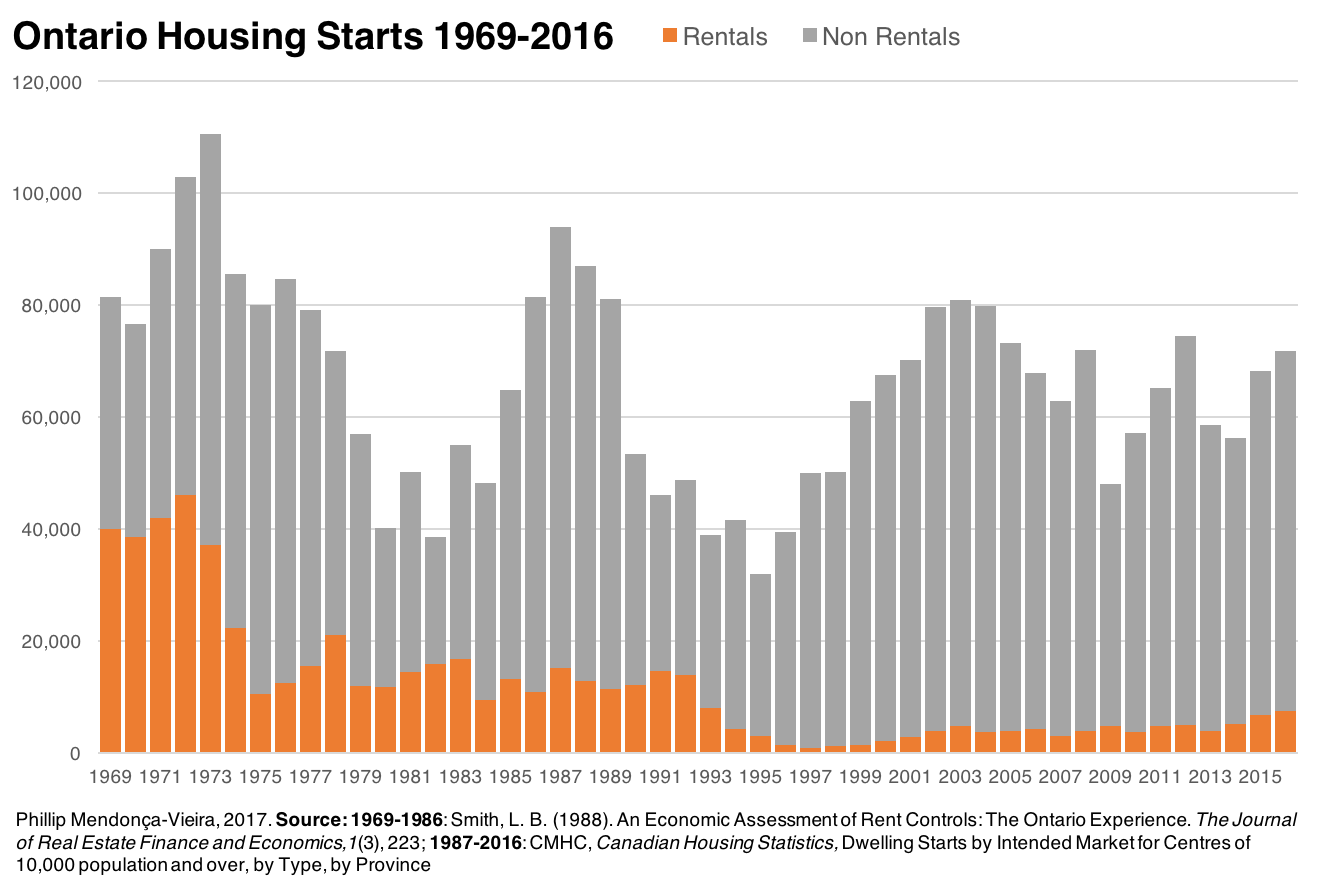
\includegraphics[width=\textwidth]{Ontario_Housing_Starts_1969-2016.png}
\caption[Ontario housing starts by intended market 1969-2016]{Ontario housing starts by intended market 1969-2016. Data from 1987 onwards is restricted to areas with over 10,000 people, and therefore undercounts total starts.}
\label{fig:figure2} 
\end{figure}

During the 1969-1974 pre-rent control period for which we have data, there were on average 32,704 unassisted rental starts per year, or about 30\% of total production. From 2009 to 2016, a period without any rent controls, Ontario averaged 5,147 new rental unit starts or a mere 10\% of total supply. 

If rent controls were the primary factor inhibiting new construction today, then surely we'd expect to see the opposite. Yet primary rental starts remain depressed.  Opponents of controls argue that developers continued to price in the risk of their reintroduction,\cite{^brescia-2005} but judged over the course of almost a generation that argument is wanting.

One downside of Smith's 1988 study is that it does not control for demographics, interest rates, recessions, etc. Rent controls could have caused record low vacancy rates by inducing higher demand -- but 1986 was also when the majority of the baby boom cohort hit the prime rental occupancy age range of 20-35.\footnote{\label{rental-demographics} The relationship between vacancy rates in Toronto and the corresponding age pyramid in Ontario is rather obvious; vacancy rates climbed in the 1990s as boomers entered the ownership market, and dipped again in the late 2000s as millennials, the next disproportionately large cohort, became of age.\cite{canada-2017}} Adequately controlling for everything is no easy task, mind you: reviewing the literature, it's a bit of an open question whether we possess the empirical data or theoretical capacity to do so properly.\footnote{\label{^lind-2003-note} Hans Lind, writing in 2003, noted both that the "[Smith (1988)] study is very crude, as there is no control for other factors." (p. 149) and that useful housing economic models are hard to develop given the required volume of empirical data (p. 151)\cite{^lind-2003}}

It's unsatisfying to merely note that the existing hypothesis doesn't fit new data. Ideally, we should be able to supply our own causal narrative. Why do we build fewer units than we did during a period of harsh rent control? For that matter, why aren't we building them like we used to in the 1960s? 

What else could be happening? While researching housing policy and statistics, I was able to identify two other big shifts that significantly impacted our housing supply. 

\subsection{The rise of the condominium}


The first happened in 1967, when Ontario legalized condominiums and created a new form of property ownership -- thereby substantially altering the economics behind multi-residential buildings.

This trend stands out pretty clearly when we graph condos compared to rentals:


\clearpage
\begin{figure}[ht]
\centering 
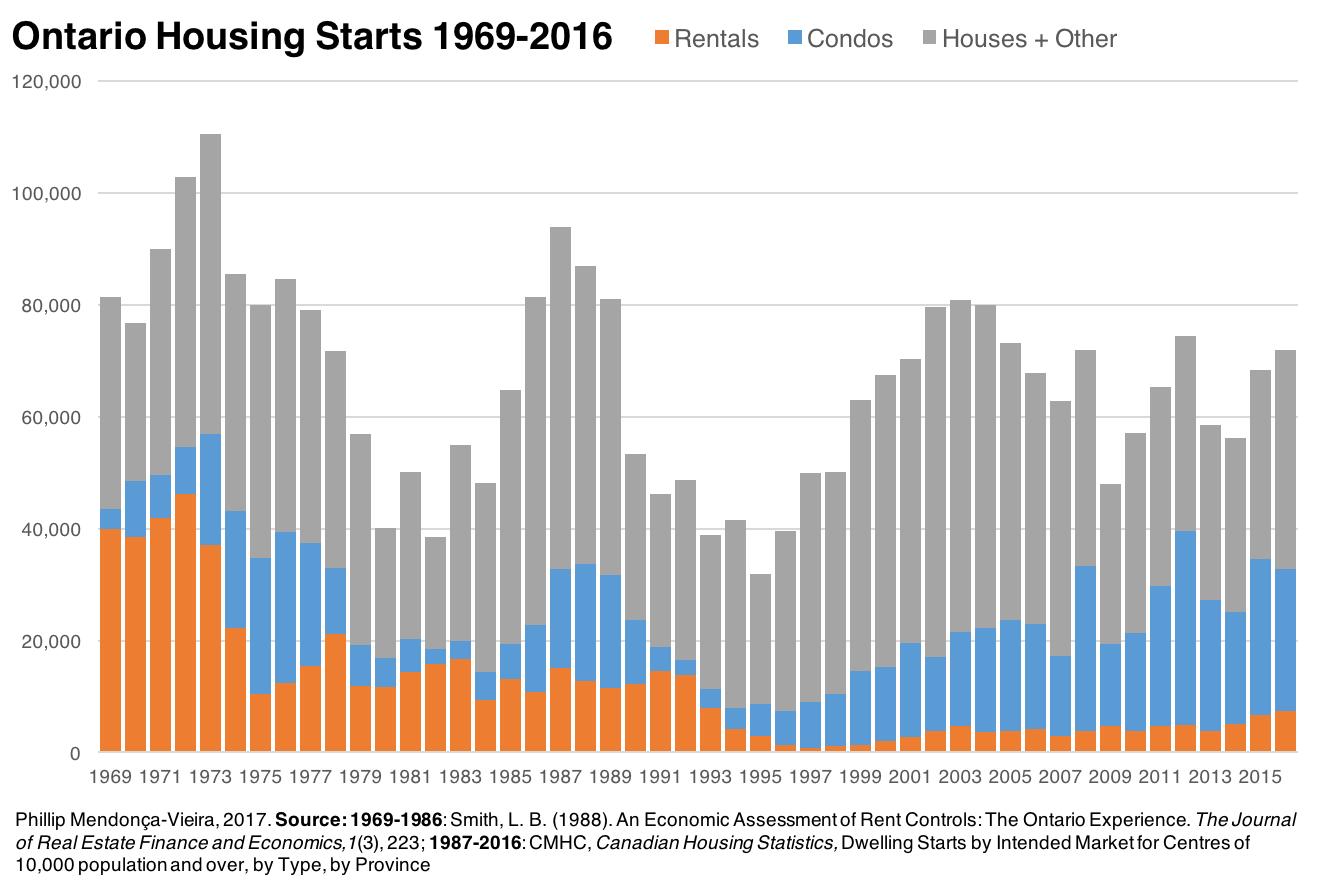
\includegraphics[width=\textwidth]{Ontario_Housing_Starts_1969-2016_With_Condos.png}
\caption[Ontario housing starts by intended market and condos 1969-2016]{Figure 2, but distinguishing condos from single, detached and other housing.
}
\label{fig:figure3} 
\end{figure}

On second thought I wondered whether looking at this data at a regional level might be misleading, since different sub-regional housing markets have differing economic conditions. As you can see from the housing mix in figure 3, Ontario was and still is aggressively subdividing and sprawling. With an abundance of available freehold land it's possible that, looking at province-wide data, we might understate the impact of condominiums. How would this look like in an already built-up area where by and large higher density developments are the only option? 

For that reason, I dug up and plotted recent and historical data from Toronto:\footnote{\label{^note-digging} CMHC's website provides convenient access only to data back to 1990. For information prior to then, you have to look it up yourself in the yearly housing statistics publications. However, the yearly publications only began to list information on starts or completions by intended market starting in  1985. In order to make the time frame being compared as similar as possible, I relied on a City of Toronto report.}

\clearpage

\begin{figure}[ht]
\centering 
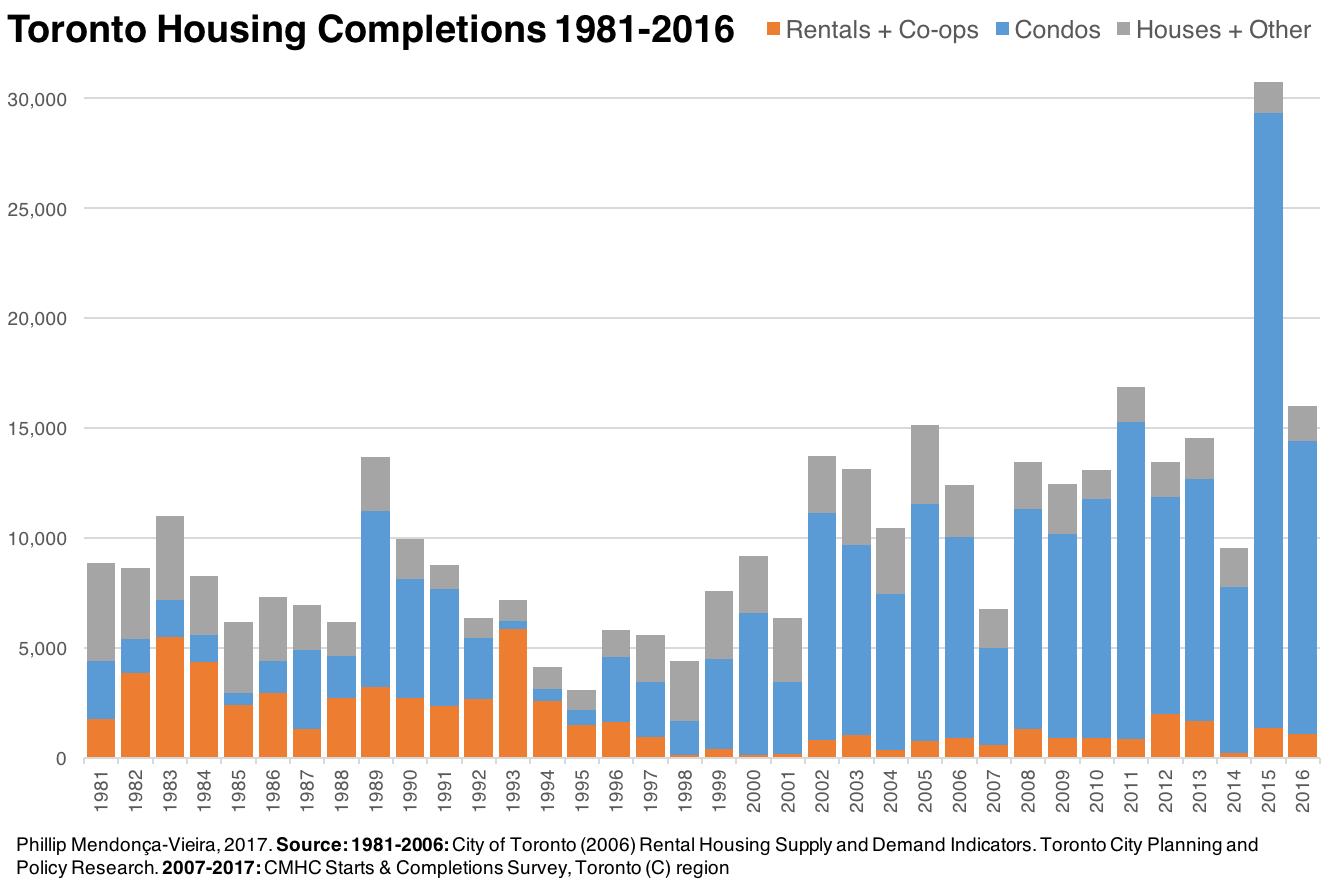
\includegraphics[width=\textwidth]{Toronto_Housing_Completions_1981-2016.png}
\caption[City of Toronto housing completions by intended market 1981-2016.]{City of Toronto housing completions by intended market 1981-2016. Note that this graph measures completions, as opposed to starts, and is therefore not directly comparable to figure 3.}
\label{fig:figure4} 
\end{figure}

Prior to the Condominium Act, apartment buildings could only be rented out or sold in their entirety. Now, for the first time, title could be given to each individual unit, greatly increasing the allowed density of privately owned housing. Condominiums immediately began to crowd out rental building investment: the first condo in Ontario was originally constructed as a rental and was converted to a condominium soon after the law came into effect.\cite{^hanes-2008} 

In 2012 Jill Black wrote a great research paper regarding the financing and economics of multi-residential housing development. She explores the incentives property developers act on and the disincentives they suffer as they choose projects to work on, and it's well worth a read. According to her research, building to rent is riskier and less profitable than building to sell.\cite{^black-2012}

Developers find building for the ownership market more attractive because with condominium projects construction doesn't begin until a majority of units are pre-sold to qualified buyers. This early-on cash stream reduces the amount of necessary debt, lowers interest repayment costs and makes it easier to obtain financing. By the time the condo units are occupied, the developer has realized their returns and freed up their equity for use in other projects.\cite{^black-2012-2}

In contrast, a rental building doesn't generate income until it's completed and therefore it's harder to assess and demonstrate its financial feasibility. This means more equity is needed to obtain more expensive, CMHC insured, financing -- equity which won't be recouped for years or decades to come.\cite{^black-2012-2} Land values, which account for 15-30\% of the cost, are thus driven by the more profitable condominium projects.\cite{^pomeroy-2001} In a way, the development of condominiums in desirable locations can lead to a kind of "Dutch disease", whereby the more profitable projects support an increase in costs and prices that make other, lower margin, projects unprofitable by comparison.\footnote{\label{^lind-2003-2}  "Very few new projects were also started in the suburbs around the year 2000, as production costs had increased faster than the willingness to pay. This can be seen as a kind of Dutch disease, where the increase in factor prices generated by some profitable sectors—the centrally located condominiums—makes other “low-margin” sectors unprofitable." Lind (2003, p. 159)}

Finally, registering as a condominium allows for a more favourable tax treatment, since multi-residential properties are discriminated against by both our sales tax regime\footnote{\label{^lampert-2016-note} Rental buildings are GST/HST exempt, as opposed to zero-rated -- meaning that unlike other businesses they can't pass on sales tax to final consumers.\cite{^lampert-2016}} and by municipal property tax rates which are set higher than ownership housing.\cite{^hswg-2001} The average tenant in Ontario pays twice the property tax rate of a homeowner, which for a hypothetical new rental building in Toronto works out to over \$200 a month in rent per tenant.\cite{^frpo-2015}

However, condominiums didn't just change supply incentives. They also changed demand. Ownership has several advantages compared to renting: a homeowner has more control over their surroundings, an easier time accumulating wealth, enjoys tax benefits (which we will soon discuss), and so on. By expanding the options for ownership, condominiums remove the highest income earners from the rental market. As a consequence, "there has been a significant fall in the demand for private renting amongst those able to pay the rents needed to generate new construction of private rented housing" and renting has increasingly become the domain of people with lower incomes.\cite{^crook-1998}

All of this conspires to make profit margins in the multi-residential investment market very narrow. What might be a suitable rate of return for an insurance company looking to operate a rental building is often insufficient for a developer to build a new one.\cite{^hswg-2001} Small shifts in financing terms, land values, costs incurred due to delays in the regulatory planning process, and taxation can have a serious impact on the feasibility of a given project.

The notion that condos crowded out rental investment is compelling, but by itself doesn't really exculpate rent controls. What if controls are just enough of a disincentive to shift the equilibrium? 

\subsection{The end of real estate tax shelters}

The other significant event occurred in 1972, when the federal government overhauled our income tax system. Seeking to make taxation more equitable, close loopholes and reorient which industries it incentivized,\cite{^budget-1971} starting in 1972 and throughout the 70s and 80s, the federal government implemented a series of reforms. 

For the first time, the government began to tax capital gains -- with the notable exception of the sale of a primary residence. The government changed the tax treatment of losses due to capital cost allowances, the rate at which capital costs can be depreciated, and it removed the ability to pool rental buildings and defer the recapture of depreciation upon sale of a property. It also prevented investors from outside the real estate business from claiming capital cost deductions or offsetting income via rental losses, and it altered how and which "soft" construction costs like architect fees, building permits, etc, can be deducted,\cite{^hswg-2001} amongst other changes.\footnote{\label{^note-on-taxes}  It's easy to understate these reforms because the true scope of the changes is a hard story to tell. There are a good half dozen different tax levers being pulled at different times: depreciation rates were altered, deductions eliminated, investment rules were changed and so on in 1972, 1974, 1978, 1981, 1986, etc. To compensate for these changes, the federal government introduced a variety of subsidies, like the Multiple Unit Residential Building in 1974, the Assisted Rental Program in 1975, etc, etc. If you want to go deep on these topics, see Clayton (1998), Housing Supply Working Group (2001), and Miron (1995), among many others cited in this article.
} \cite{^clayton-1998} \cite{^miron-1995}

In practical terms this meant that purpose-built rental buildings became a far less attractive investment class while homeownership became far more attractive. Taxing all capital gains except primary residences, in addition to the variety of demand and supply side incentives and subsidies being offered at the time, is a considerable enticement for diverting money into homeownership. With regard to rentals, being able to depreciate a building tax-wise at a faster rate than its actual economic depreciation can have a large impact on after-tax returns.\cite{^hswg-2001} Rental buildings become more profitable over time, as inflation and debt repayment lowers ongoing operating costs; prior to these reforms, high-earning professionals could use losses generated by rental properties to offset their higher marginal tax rates, and they could use liberal capital cost allowance rates to defer income tax until they sold their property.\cite{^miron-1995}

Additionally, in 1991 the Goods and Services Tax was introduced (and later, harmonized in most provinces), which increased the sales tax burden on new construction by almost 70 per cent.\cite{^enemark-2017} Whereas before only the building materials used in the construction of a rental building had a sales tax, now the full value of the building was subject to a 7 percent charge (though, lower today).\cite{^clayton-1998-2} Renters don't pay GST/HST on their rent, which means that developers are stuck with input credits they can't use thereby "stranding" tax costs.\cite{^lampert-2016}

Marion Steele, writing in 1993, argued that these reforms, coupled with contemporary macro economic conditions, incentivized small scale landlording. The 1970s and 1980s featured high inflation and unprecedented housing price booms which made expected capitals gains "the dominating motivation of investors". Capital gains, in turn, are more valuable to high-income individuals than they are to corporations, whose marginal tax rates are lower.\cite{^steele-1993} Before, developers built large scale schemes for their own investment, and smaller schemes for sale to high-income individuals or their syndicates. But now these tax changes prompted developers to leave the industry,\cite{^crook-1998-2} and drew investors to dwelling structures that were easier to sell and whose conversion to ownership tenure was unrestricted: houses, duplexes, etc, and condominium units.\cite{^steele-1993}

These changes were made with little, if any, regard for their adverse consequences for our housing policy goals,\cite{^clayton-1998} and given that the "Great Apartment Boom" of the 1960s ended shortly thereafter suggests that the effect of these changes was substantial.\cite{^miron-1995}


\begin{figure}[ht]
\centering 
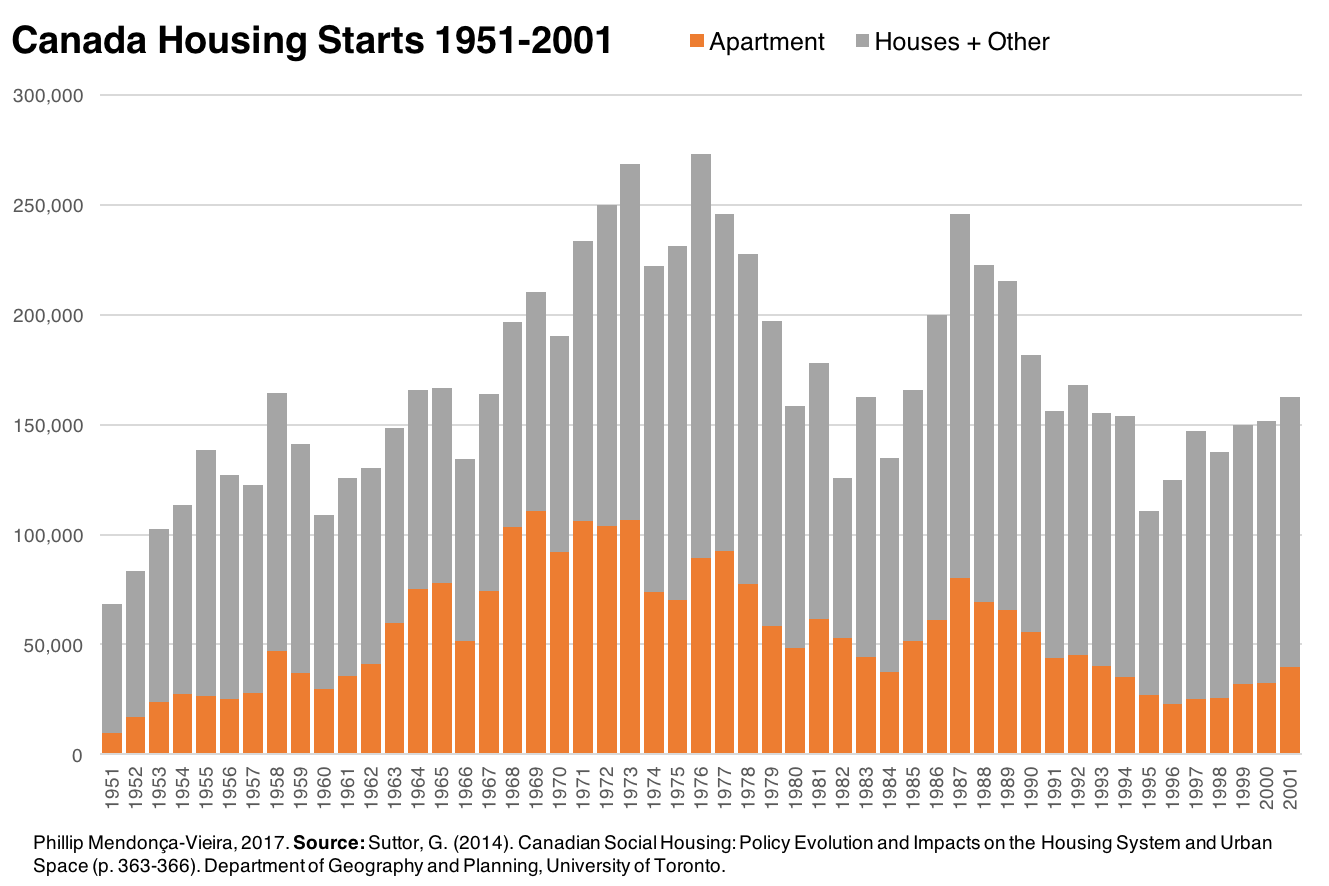
\includegraphics[width=\textwidth]{Canada_Housing_Starts_1951-2001.png}
\caption[Canada housing starts by structure type 1951-2001]{Note that these categories describe physical structures, i.e. "apartment" includes both duplexes, triplexes, etc and the large towers we today find synonymous with condominiums. We built more (almost entirely rental) apartment buildings in 1968 than we built (mostly condos) apartment buildings in 2001 (or 2016, for that matter).}
\label{fig:figure5} 
\end{figure}


Various Trudeau governments recognized there were consequences from changing the Income Tax Act and tried to do something about it. The Multi-Unit Residential Building incentive (1974-1979, 1981) re-enabled the use of rental investment as a tax shelter. The Assisted Rental Program (1974-1979, 1981) gave subsidized mortgages to developers in exchange for below-market rents. The Canada Rental Supply Program (1981-1984) provided interest-free loans for up to fifteen years. The list goes on.\cite{^goldberg-1985} \cite{^suttor-2009}

Besides our declining rental housing starts, we have one other piece of evidence: the United States' current tax regime as applied to rental buildings is broadly similar to how we did things pre-1972.\cite{^clayton-1998-3} Though we can't compare them directly -- Canada and the US are very different places -- consider the example of Seattle and Vancouver. While Vancouver is experiencing a furious condo boom, taking up to 60\% of housing starts, the vast majority of new units in Seattle are apartment buildings.\footnote{\label{^nota-bene}  Ah ha, you say, but rent controls are \emph{illegal} in Washington State. Yet condos don't get built because of prohibitive building standards. It's complicated and hard to compare!} \cite{^morales-2017}


\subsection{In review}

Commentators argue that rent controls are harmful because they remove new primary rental supply from the market, and therefore exacerbate the problem of low vacancies. However, in 1998 the province permanently exempted new construction from rent controls.

Since then investment in units intended for the rental market continues to be depressed. Instead, I argue that two other concurrent policy changes can better explain this trend. The first was the legalization of condominiums, which crowded out investment in rental buildings. The second were income and sales tax reforms, which has reduced the profitability of rental buildings.

Of course, there are many other factors and angles we haven't looked at. We have not controlled for the huge impacts of fluctuating interest rates, demographic trends, surging land prices, etc. Tenants are further discriminated by municipal property taxes and exclusionary zoning restrictions. Yet given the timing of these changes it seems fair to say that rent controls qua rent controls are not the main disincentive operating today.

But if Ontario's rent controls probably did not impact the supply of new housing, what else can we say about them? How does this evidence fit into the theoretical basis behind most economists' criticism of rent controls? What evidence do we have from other jurisdictions? What other criticisms are misguided — and which ones are well founded?


%------------------------------------------------

%------------------------------------------------

\section*{Conclusion}


\begin{enumerate}
\item First numbered list item
\item Second numbered list item
\end{enumerate}

Donec luctus tincidunt mauris, non ultrices ligula aliquam id. Sed varius, magna a faucibus congue, arcu tellus pellentesque nisl, vel laoreet magna eros et magna. Vivamus lobortis elit eu dignissim ultrices. Fusce erat nulla, ornare at dolor quis, rhoncus venenatis velit. Donec sed elit mi. Sed semper tellus a convallis viverra. Maecenas mi lorem, placerat sit amet sem quis, adipiscing tincidunt turpis. Cras a urna et tellus dictum eleifend. Fusce dignissim lectus risus, in bibendum tortor lacinia interdum.

%----------------------------------------------------------------------------------------
%	BIBLIOGRAPHY
%----------------------------------------------------------------------------------------


\begin{thebibliography}{9}

\bibitem{ltb-2017}
 Landlord and Tenant Board. (2017, May). Brochure: A Guide to the Residential Tenancies Act. Retrieved September 29, 2017, from \href{http://www.sjto.gov.on.ca/documents/ltb/Brochures/Guide\%20to\%20RTA\%20(English).html}{sjto.gov.on.ca}

 \bibitem{^mcgrath-skepticism}
  McGrath, J. (2017, March 22). Ontario needs a rental rethink, but should tread carefully. Retrieved August 17, 2017, from \href{https://tvo.org/article/current-affairs/ontario-needs-a-rental-rethink-but-should-tread-carefully}{tvo.org}

\bibitem{^mcfarland-vigorous}
  McFarland, J. (2017, April 4) `Exact opposite of what is needed': CIBC slams Ont. rent-control rules. Retrieved August 17, 2017, from \href{https://www.theglobeandmail.com/real-estate/toronto/new-ontario-rent-control-rules-exact-opposite-of-what-is-needed-analyst-warns/article34569276/}{theglobeandmail.com}


\bibitem{^gee-2017}
 Gee, M. (2017, April 20). Rent control isn't the solution to Ontario's housing problem. Retrieved September 12, 2017, from \href{https://beta.theglobeandmail.com/news/toronto/rent-control-isnt-the-solution-to-ontarios-housing-problem/article34753102/}{theglobeandmail.com}

\bibitem{^tal-2017}
 Tal, B. (2017, April 4). Rent Control—The Wrong Medicine. Retrieved September 12, 2017, from \href{https://economics.cibccm.com/economicsweb/cds?ID=2595&TYPE=EC_PDF}{economics.cibccm.com}

\bibitem{selley}
 Selley, C. (2017, March 21). Chris Selley: Rent control is a bad solution to the wrong problem. Retrieved September 12, 2017, from \href{http://nationalpost.com/news/toronto/chris-selley-rent-control-is-a-bad-solution-to-the-wrong-problem}{nationalpost.com}

\bibitem{thesun}
 Lafleur, S., \& Filipowicz, J. (2017, April 15). Rent controls wrong answer to housing crisis. Retrieved September 12, 2017, from \href{http://www.torontosun.com/2017/04/15/rent-controls-wrong-answer-to-housing-crisis}{torontosun.com}

\bibitem{cbc-squeeze}
  McGillivray, K. (2017, April 05). Ontario second-worst economy for young people in Canada: report. Retrieved September 12, 2017, from \href{http://www.cbc.ca/news/canada/toronto/generation-squeeze-ontario-economy-1.4054589}{cbc.ca}
  
\bibitem{cbc-martin}
  Martin, S. (2017, February 22). No fixed address: How I became a 32-year-old couch surfer. Retrieved September 29, 2017, from \href{http://www.cbc.ca/news/canada/toronto/no-fixed-address-how-i-became-a-32-year-old-couch-surfer-1.3985771}{cbc.ca}

\bibitem{tgam-jaafari}
  Jaafari, J. D. (2017, April 14). Toronto tenants crushed by rent hike exemptions. Retrieved September 29, 2017, from \href{https://beta.theglobeandmail.com/news/toronto/toronto-tenants-crushed-by-rent-hike-exemptions/article33806825/}{theglobeanmail.com}

\bibitem{mercer-2017}
  Mercer, G. (2017, May 13). Tenants sound alarm on creeping rents. Retrieved October 31, 2017, from \href{https://www.therecord.com/news-story/7312772-tenants-sound-alarm-on-creeping-rents/}{therecord.com}

\bibitem{toronto-2006}
  City of Toronto (2006) \href{https://www1.toronto.ca/city_of_toronto/social_development_finance__administration/files/pdf/housing_rental.pdf}{Rental Housing Supply and Demand Indicators}. Toronto City Planning and Policy Research

\bibitem{^smith-1983}
 Smith, L. B. (1983). The Crisis in Rental Housing: A Canadian Perspective. The Annals of the American Academy of Political and Social Science, 465(1), p. 3-4, 58-75. doi:10.1177/0002716283465001006

\bibitem{^smith-1988}
  Smith, L. B. (1988). An economic assessment of rent controls: The Ontario experience. The Journal of Real Estate Finance and Economics, 1(3), 217-231. doi:10.1007/bf00658918A

\bibitem{^miron-1995}
 Miron, J. R. (1995). Private Rental Housing: The Canadian Experience. Urban Studies, 32(3), 579-604. doi:10.1080/00420989550012988

\bibitem{^august-2017}
  August, M., Walks, A. (2017) Gentrification, suburban decline, and the financialization of multi-family rental housing: The case of Toronto. http://dx.doi.org/10.1016/j.geoforum.2017.04.011

\bibitem{rent-control-city-report}
  Staff report for information on Tenant Issues Related to the RTA 1 (Rep. pg 2-3). (2013, October 15). Retrieved August 28, 2017, from \href{http://www.toronto.ca/legdocs/mmis/2013/ex/bgrd/backgroundfile-63467.pdf}{toronto.ca}

\bibitem{^smith-2003}
 Smith, L. B. (2003). Intertenancy Rent Decontrol in Ontario. Canadian Public Policy / Analyse de Politiques, 29(2), 213. doi:10.2307/3552456

\bibitem{^brescia-2005}
 Brescia, V. (2005). The Affordability of Housing in Ontario: Trends, Causes, Solutions (p. 31).

\bibitem{canada-2017}
  Government of Canada (2017, May 01). Historical Age Pyramid. Retrieved October 20, 2017, from \href{http://www12.statcan.gc.ca/census-recensement/2016/dp-pd/pyramid/pyramid.cfm?geo1=35\&type=1}{statcan.gc.ca}

\bibitem{^lind-2003}
Lind, H. (2003). Rent regulation and new construction: With a focus on Sweden 1995-2001. Swedish Economic Policy Review, (10), 135-167.

\bibitem{^black-2012}
 Black, J. (September 2012). The Financing and Economics of Affordable Housing: Development Incentives and Disincentives to Private-Sector Participation (p. 8-9, 20), Cities Centre, University of Toronto

\bibitem{^black-2012-2}
 Black (2012, p. 8-9)

\bibitem{^hanes-2008}
  Hanes, T. (2008, February 23). Happy 40th. Retrieved September 18, 2017, from \href{https://www.thestar.com/news/2008/02/23/happy_40th.html}{thestar.com}

\bibitem{^pomeroy-2001}
 Pomeroy, S. (2001, October). Toward a Comprehensive Affordable Housing Strategy for Canada (p. 15).

\bibitem{^lampert-2016}
Lampert, G. (2016). Encouraging Construction and Retention of Purpose-Built Rental Housing in Canada: Analysis of Federal Tax Policy Options (p. 6). 

\bibitem{^hswg-2001}
 Housing Supply Working Group. (2001, May) Affordable Rental Housing Supply: The Dynamics of the Market and Recommendations for Encouraging New Supply, p. 9-14, 17-18

\bibitem{^frpo-2015}
 Federation of Rental-housing Providers of Ontario (2015) Removing Barriers to New Rental Housing in Ontario (p. 18)

\bibitem{^crook-1998} Crook, T. (1998) The Supply of Private Rented Housing in Canada. Netherlands Journal of of Housing and the Built Environment, 13(3), 339

\bibitem{^budget-1971}
  Benson, E. J. (1971, June 18) Budget speech delivered by the Honourable E. J. Benson Minister of Finance and Member of Parliament for Kingston and The Islands. Retrieved from \href{http://www.budget.gc.ca/pdfarch/1971-sd-eng.pdf}{budget.gc}

\bibitem{^clayton-1998}
 Clayton, F. (1998, November) Economic Impact of Federal Tax Legislation on the Rental Housing Market in Canada (p. i, 9-12) Canadian Federation of Apartment Associations - Fédération Canadienne des Associations de Propriétaires Immobiliers

\bibitem{^enemark-2017}
  Enemark, T. (2017, July 06). Fastest Way to More Rental Housing? Tax Changes. Retrieved September 12, 2017, from \href{https://thetyee.ca/Opinion/2017/07/06/Tax-Changes-More-Rental-Housing/}{thetyee.ca}

\bibitem{^steele-1993}
  Steele, M. (1993) Conversions, Condominiums and Capital Gains: The Transformation of the Ontario Rental Housing Market. Urban Studies 30(1), 103-126

\bibitem{^crook-1998-2} Crook (1998, p. 335-336)

\bibitem{^goldberg-1985}
 Goldberg, M. A., \& Mark, J. H. (1985). The Roles of Government in Housing Policy A Canadian Perspective and Overview. Journal of the American Planning Association, 51(1), 35-36. doi:10.1080/01944368508976798

\bibitem{^suttor-2009}
 Suttor, G. (2009). Rental Paths from Postwar to Present: Canada Compared (p. 39-40, Research Paper 218). Toronto: Cities Centre University of Toronto.

\bibitem{^clayton-1998-2}
 Clayton (1998, p. 9, 32-33)
  

\bibitem{^clayton-1998-3}
 Clayton (1998, p. 14, 28) 

\bibitem{^morales-2017}
  Morales, M. (2017, August 14). Why Seattle Builds Apartments, but Vancouver, BC, Builds Condos. Retrieved September 13, 2017, from \href{http://www.sightline.org/2017/08/14/why-seattle-builds-apartments-but-vancouver-bc-builds-condos/}{sightline.org}

% part two

\bibitem{^arnott-1995}
   Arnott, R. (1995). Time for Revisionism on Rent Control? Journal of Economic Perspectives,9(1), 100-102, 112-115. doi:10.1257/jep.9.1.99

\bibitem{^lind-2001}
  Lind, H. (2001). Rent Regulation: a Conceptual and Comparative Analysis. European Journal of Housing Policy, 1(1), 41-57. doi:10.1080/14616710110036436

\bibitem{^nycrgb-2016}
  New York City Rent Guidelines Board. (2016, September 23). Rent Control FAQ. Retrieved October 30, 2017, from \href{http://www.housingnyc.com/html/resources/faq/rentcontrol.html}{housingnyc.com}

\bibitem{^curbed-2017}
  Nonko, E. (2017, August 28). Rent control vs. rent stabilization in NYC, explained. Retrieved October 30, 2017, from \href{https://ny.curbed.com/2017/8/28/16214506/nyc-apartments-housing-rent-control}{ny.curbed.com}

\bibitem{^arnott-2003}
  Arnott, R (2003). Tenancy Rent Control. Swedish Economic Policy Review, (10), 98

\bibitem{^macfarlane-2001}
  Mcfarlane, A. (2001). Rent Stabilization and the Long-Run Supply of Housing. SSRN Electronic Journal. doi:10.2139/ssrn.283336

\bibitem{^black-2012-4}
  Black, J. (September 2012). The Financing and Economics of Affordable Housing: Development Incentives and Disincentives to Private-Sector Participation (p. 8-12), Cities Centre, University of Toronto

\bibitem{^tait-2017}
  Tait, S. (2017, April 30). Ontario’s Fair Housing Plan \& Purpose-Built Rental Development. Retrieved September 14, 2017, from \href{https://www.linkedin.com/pulse/ontarios-fair-housing-plan-purpose-built-rental-development-sean-tait/}{linkedin.com}

\bibitem{^marr-2017}
  Marr, G. (2017, July 18). Rent controls, no worries. Developer unveils major apartment complex in downtown Toronto. Retrieved September 14, 2017, from \href{http://business.financialpost.com/real-estate/property-post/one-of-the-best-assets-classes-major-landlord-expects-rental-apartment-demand-to-remain-strong-despite-rent-controls}{business.financialpost.com}

\bibitem{^grant-2011}
  Grant, H. (2011, January 31). An Analysis of Manitoba’s Rent Regulation Program and the Impact on the Rental Housing Market. Manitoba Family Services and Consumer Affairs

\bibitem{^ambrosius-2015}
   Ambrosius, J. D., Gilderbloom, J. I., Steele, W. J., Meares, W. L., \& Keating, D. (2015). Forty years of rent control: Reexamining New Jersey’s moderate local policies after the great recession. Cities: The International Journal of Urban Policy and Planning, 49, 121-133. doi:10.1016/j.cities.2015.08.001

\bibitem{^haines-2017}
  Haines, G. (2017, April 28). Making Cents of Ontario’s Rent Regulation: Assessing the Financial Impact of Rent Control and Developer Incentives. Ryerson City Building Institute.

\bibitem{^ambrosius-2015-2}
  Ambrosius et al (2016, p. 129-130)

\bibitem{^grant-2011-2}
  Grant (2011, p. 24)

\bibitem{^denton-1993}
  Denton, F. T., Feaver, C. H., Muller R. A., Robb, A. L., Spencer, B. G. (1993). Testing Hypotheses About Rent Control: Final Report. Ottawa: CMHC.

\bibitem{^lazzarin-1990}
  Lazzarin, C. C. (1990). Rent Control and Rent Decontrol in British Columbia: A Case Study of the Vancouver Rental Market, 1974 to 1989. University of British Columbia.

\bibitem{^sims-2007}
  Sims, D. P. (2007). Out of control: What can we learn from the end of Massachusetts rent control? Journal of Urban Economics, 61(1), 129-151. doi:10.1016/j.jue.2006.06.004

\bibitem{^diamond-2017}
   Diamond, R., McQuade, T., \& Qian, F. (2017). The Effects of Rent Control Expansion on Tenants, Landlords, and Inequality: Evidence from San Francisco.

\bibitem{^mclaughlin-2016}
  McLaughlin, R. (2016, August 31). Rich City, Poor City: How Housing Supply Drives Regional Economic Inequality. Retrieved October 31, 2017, from \href{https://www.trulia.com/blog/trends/rich-city-poor-city/}{trulia.com}

\bibitem{^torres-2017}
  Torres, B. (2017, April 28). Housing’s tale of two cities: Seattle builds, S.F. lags. Retrieved October 30, 2017, from \href{https://www.bizjournals.com/sanfrancisco/news/2017/04/28/san-francisco-seattle-housing-production-pipelines.html}{bizjournals.com}

\bibitem{^hswg-final}
  Lampert, G., Pomeroy, S., \& Bradley, R. (2002). Creating a Positive Climate for Rental Housing Development Through Tax and Mortgage Insurance Reforms: The Second Report of the Housing Supply Working Group (p. 7). Toronto: Ministry of Municipal Affairs and Housing.

\bibitem{^brescia-2005-3}
  Brescia (2005, p. 7-8)

\bibitem{^brescia-2005-2}
   Brescia (2005, p. 27)

% part three
\bibitem{^jenkins-2009}
  Jenkins, B. (2009, January) Rent Control: Do Economists Agree? Econ Journal Watch, 6(1), 73-112

\bibitem{^arnott-2003-2}
  Arnott (2003, p. 111)

\bibitem{^yee-1989}
  Yee, G. (1989) Rationales for Tenant Protection and Security of Tenure, Journal of Law and Social Policy (5), p. 48, 50

\bibitem{^economist-1998}
  The morning after. (1998, May 02). Retrieved October 31, 2017, from \href{http://www.economist.com/node/161526}{economist.com}

\bibitem{^hulchanski-laissez}
  Hulchanski (1984, p. 27)

\bibitem{^brescia-2005-4}
  Brescia (2005, p. 26)

\bibitem{^suttor-abridged}
  Suttor, G. (2016) Canadian Social Housing: Policy Evolution and Program Periods, p. 12

\bibitem{^hulchanski-bulletin38}
  Hulchanski, J. D. (2007, September) Canada’s Dual Housing Policy Assisting Owners, Neglecting Renters, University of Toronto Centre for Urban and Community Studies

\bibitem{^yorke-2015}
  Yorke, B. (2015, December 10). The Tenant Movement in B.C. from 1968 to 1978. Retrieved September 20, 2017, from \href{http://themainlander.com/2012/11/09/the-tenant-movement-in-b-c-from-1968-to-1978/}{themainlander.com}

\bibitem{^hulchanski-tenant-rights}
   Hulchanski (1984, p. 74-75)

 \bibitem{^hulchanski-1984}
    Hulchanski, J. D. (1984) Market Imperfections and the Role of Rent Regulations in the Residential Rental Market, Toronto: Ontario Commission of Inquiry into Residential Tenancies, Research Study No. 6.

\bibitem{^mcardle-2017}
  McArdle, M. (2017, June 16). Beware of Blaming Government for London Tower Fire. Retrieved September 12, 2017, from \href{https://www.bloomberg.com/view/articles/2017-06-16/beware-of-blaming-government-for-london-tower-fire}{bloomberg.com}

\bibitem{^fire-deaths}
  Fire Death Rates. (2016, December). Retrieved September 12, 2017, from \href{https://www.mcscs.jus.gov.on.ca/english/FireMarshal/MediaRelationsandResources/FireStatistics/OntarioFatalities/FireDeathRate/stats\_death\_rate.html}{mcscs.jus.gov.on.ca}

\bibitem{^cowen-2007}
  Cowen, T. (2007, December). Public Goods. Retrieved November 02, 2017, from \href{http://www.econlib.org/library/Enc/PublicGoods.html}{econlib.org}

\bibitem{^galea-2016}
  Quote is by John Kenneth Galbraith via Galea, S. (2016, January 10). Public Health as a Public Good | SPH | Boston University. Retrieved November 02, 2017, from \href{https://www.bu.edu/sph/2016/01/10/public-health-as-a-public-good/}{bu.edu}

\bibitem{^desmond}
   Desmond, M. (2016). Evicted: Poverty and Profit in the American City. Crown Books. p. 70, 296-298.

\bibitem{^mcgrath-2017}
  McGrath, J. (2017, July 14). There's life outside Toronto, but leaving the city is harder than it used to be. Retrieved September 13, 2017, from \href{http://tvo.org/article/current-affairs/the-next-ontario/theres-life-outside-toronto-but-leaving-the-city-is-harder-than-it-used-to-be}{tvo.org}

\bibitem{^waldegrave-2016}
   Waldegrave, C., Urbanová, M. (2016, November) Social and Economic Impacts of Housing Tenure. New Zealand Housing Foundation.

\bibitem{^tal-rent-2017}
  Tal, B. (2017, March 15). GTA Housing—Rent Must be Part of the Solution. Retrieved September 1, 2017, from \href{https://economics.cibccm.com/economicsweb/cds?ID=2475\&TYPE=EC\_PDF}{economics.cibccm.com}

\bibitem{^census-2011}
  Statistics Canada (2017, May 3) Census concepts: A profile of the City of Toronto, Toronto Census 2016 Community Planning Session.

\bibitem{^carrick-2017}
  Carrick, R. (2017, November 02). Accept it, your children may grow up to be renters. Retrieved November 02, 2017, from \href{https://beta.theglobeandmail.com/globe-investor/personal-finance/household-finances/accept-it-your-children-may-grow-up-to-be-renters/article36806999/}{theglobeandmail.com}

\bibitem{^suttor-2017}
  Suttor, G., \& Leon, S. (2017, October 27). 6 Toronto Rental Housing Highlights in the 2016 Census. Retrieved November 7, 2017, from \href{http://www.wellesleyinstitute.com/housing/6-toronto-rental-housing-highlights-in-the-2016-census}{wellesleyinstitute.com}


\end{thebibliography}




\bibliographystyle{unsrt}

\bibliography{sample}

%----------------------------------------------------------------------------------------

\end{document}
